% Options for packages loaded elsewhere
\PassOptionsToPackage{unicode}{hyperref}
\PassOptionsToPackage{hyphens}{url}
%
\documentclass[
]{article}
\usepackage{lmodern}
\usepackage{amssymb,amsmath}
\usepackage{ifxetex,ifluatex}
\ifnum 0\ifxetex 1\fi\ifluatex 1\fi=0 % if pdftex
  \usepackage[T1]{fontenc}
  \usepackage[utf8]{inputenc}
  \usepackage{textcomp} % provide euro and other symbols
\else % if luatex or xetex
  \usepackage{unicode-math}
  \defaultfontfeatures{Scale=MatchLowercase}
  \defaultfontfeatures[\rmfamily]{Ligatures=TeX,Scale=1}
\fi
% Use upquote if available, for straight quotes in verbatim environments
\IfFileExists{upquote.sty}{\usepackage{upquote}}{}
\IfFileExists{microtype.sty}{% use microtype if available
  \usepackage[]{microtype}
  \UseMicrotypeSet[protrusion]{basicmath} % disable protrusion for tt fonts
}{}
\makeatletter
\@ifundefined{KOMAClassName}{% if non-KOMA class
  \IfFileExists{parskip.sty}{%
    \usepackage{parskip}
  }{% else
    \setlength{\parindent}{0pt}
    \setlength{\parskip}{6pt plus 2pt minus 1pt}}
}{% if KOMA class
  \KOMAoptions{parskip=half}}
\makeatother
\usepackage{xcolor}
\IfFileExists{xurl.sty}{\usepackage{xurl}}{} % add URL line breaks if available
\IfFileExists{bookmark.sty}{\usepackage{bookmark}}{\usepackage{hyperref}}
\hypersetup{
  pdftitle={Predicting IMBD Scores},
  pdfauthor={Shivani Dedhia, Akhila Pamukuntla, Nafis Chowdhury, Akshita Jain},
  hidelinks,
  pdfcreator={LaTeX via pandoc}}
\urlstyle{same} % disable monospaced font for URLs
\usepackage[margin=1in]{geometry}
\usepackage{graphicx,grffile}
\makeatletter
\def\maxwidth{\ifdim\Gin@nat@width>\linewidth\linewidth\else\Gin@nat@width\fi}
\def\maxheight{\ifdim\Gin@nat@height>\textheight\textheight\else\Gin@nat@height\fi}
\makeatother
% Scale images if necessary, so that they will not overflow the page
% margins by default, and it is still possible to overwrite the defaults
% using explicit options in \includegraphics[width, height, ...]{}
\setkeys{Gin}{width=\maxwidth,height=\maxheight,keepaspectratio}
% Set default figure placement to htbp
\makeatletter
\def\fps@figure{htbp}
\makeatother
\setlength{\emergencystretch}{3em} % prevent overfull lines
\providecommand{\tightlist}{%
  \setlength{\itemsep}{0pt}\setlength{\parskip}{0pt}}
\setcounter{secnumdepth}{-\maxdimen} % remove section numbering

\title{Predicting IMBD Scores}
\author{Shivani Dedhia, Akhila Pamukuntla, Nafis Chowdhury, Akshita Jain}
\date{}

\begin{document}
\maketitle

\hypertarget{sta-9750-final-project}{%
\subsection{STA 9750 Final Project}\label{sta-9750-final-project}}

\hypertarget{hypothesis}{%
\subsection{Hypothesis}\label{hypothesis}}

\hypertarget{introduction}{%
\subsection{Introduction}\label{introduction}}

Many factors make a movie successful. Some of the factors include user
reviews, budget of the movie, actor's and director's popularity. We will
find out which factor has the most impact on a movie's success and
profitability.

We have the IMDB 5000 movie dataset
(\url{https://www.kaggle.com/suchitgupta60/IMDB-data}), which has 28
variables, 5043 movies across 100 years from 66 countries. There are
many variables in the dataset such as Director, Actors, Duration, Gross,
Budget, Genres, Facebook Likes, etc.

We will be using some of the modeling techniques with associated
visualizations to identify the most important variables that impact the
success and ratings of the movie along with their profitability.

\hypertarget{data-exploration}{%
\subsection{Data Exploration}\label{data-exploration}}

After cleaning the data, we narrowed our scope of model to 26 variables
and 3806 rows. We choose to remove some features such as aspect ratio,
imdb movie link and color as they reduce the quality of our data and are
less important to our analysis.

Movies having IMDB rating above 7.5 are considered to be highly
recommended. Majority of the movies are rated 7.6 with only a handful
rated above 9 as per the distribution shown below. The highest rating
received by one movie is 9.3.

IMDB offers a scoring scale that allows users to rate films on a scale
of one to ten. It indicates that submitted scores are filtered and
weighted in various ways in order to produce a weighted mean that is
displayed for each movie.

Majority of the movies are between the range of 6.5 to 7.7 which is
considered as an average IMDB score. The histogram closely fits a normal
distribution.

However, there are only a handful of phenomenal movies which are rated
above 8.

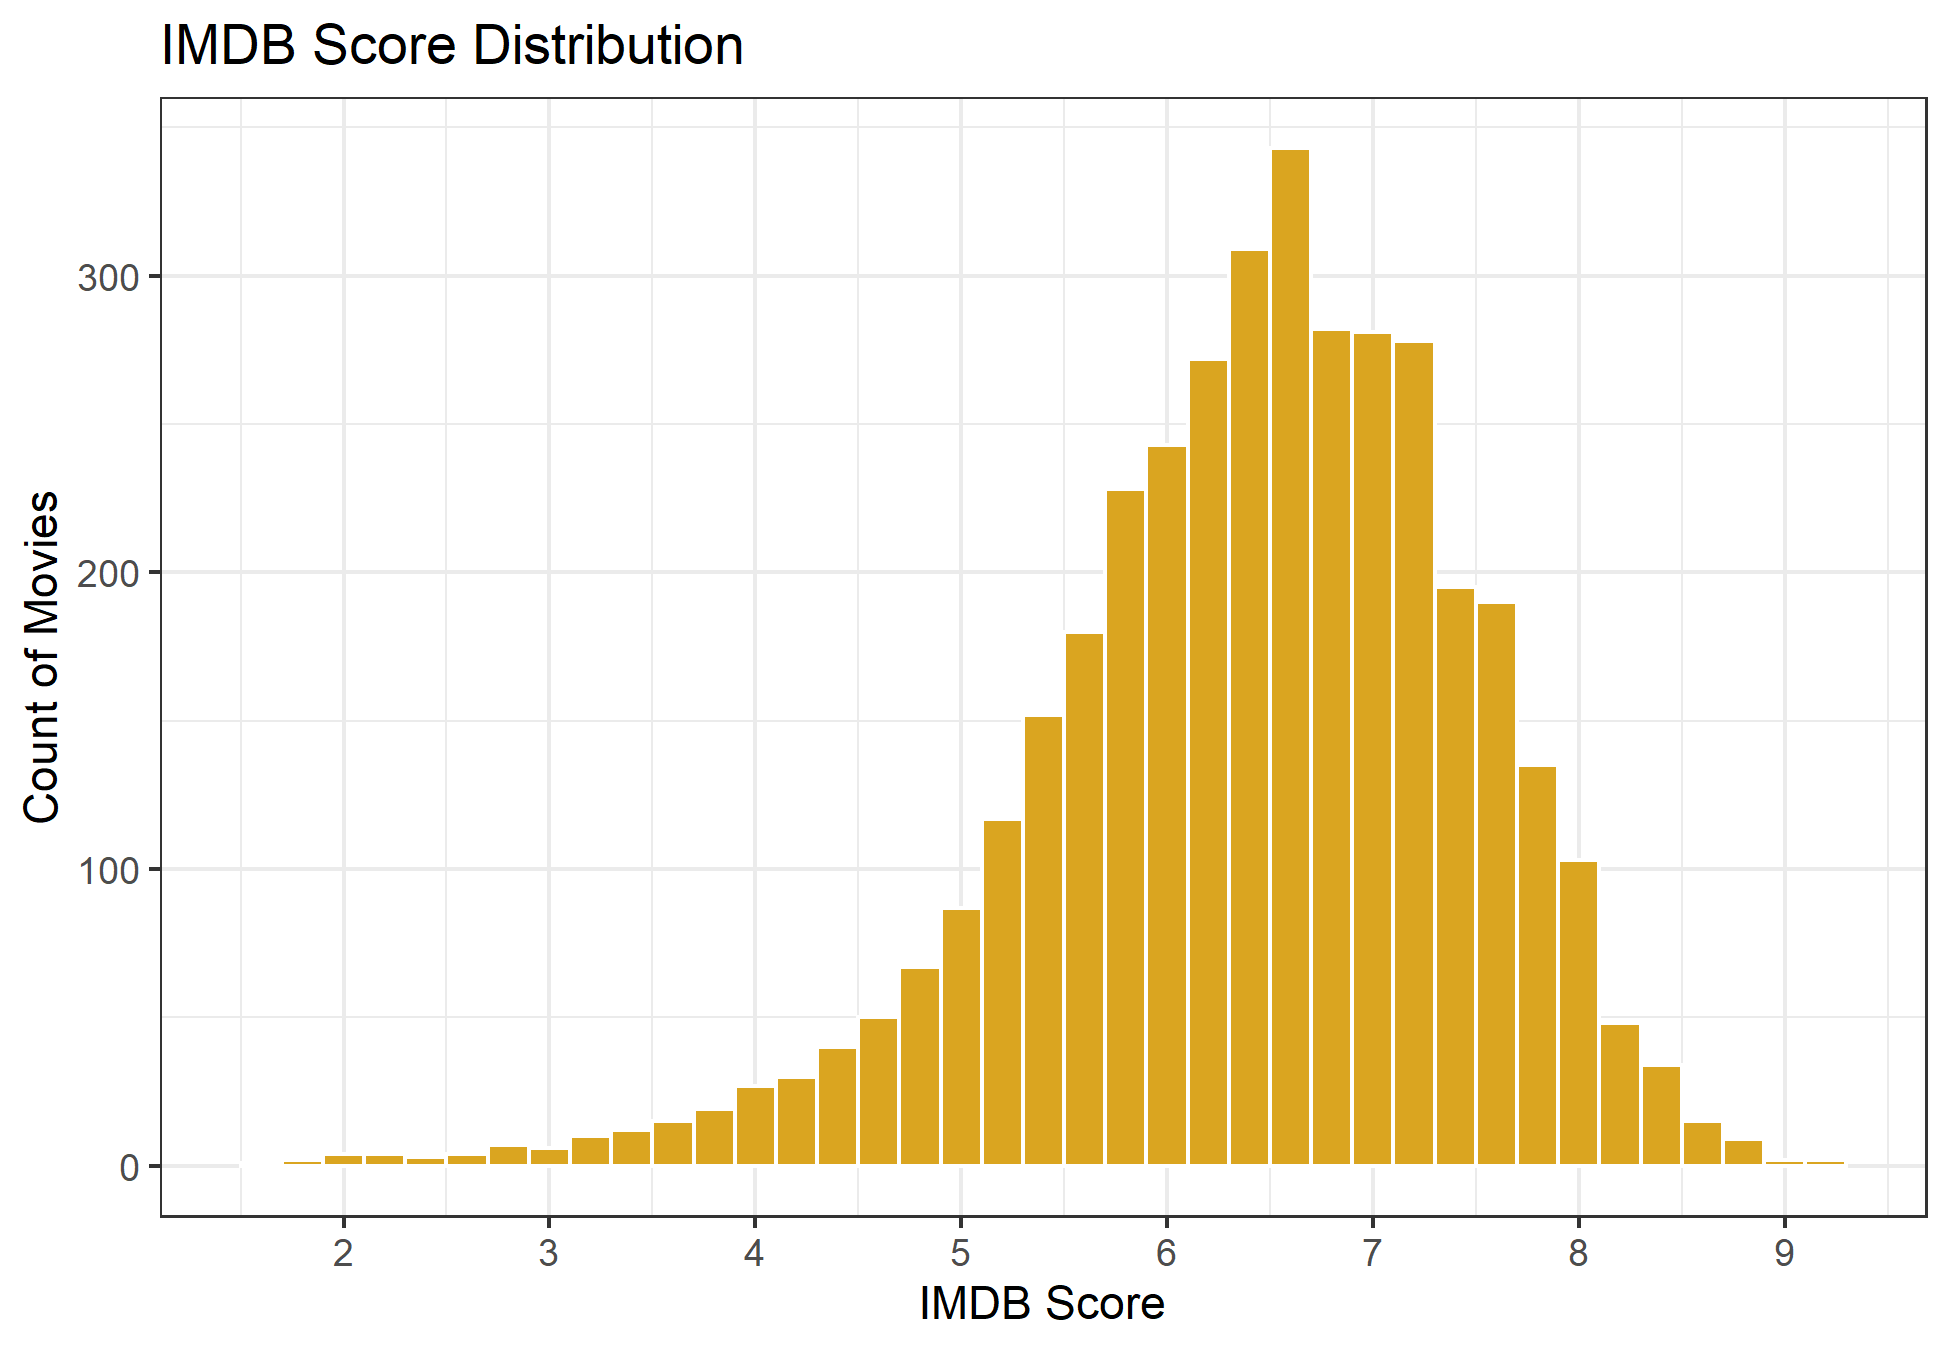
\includegraphics[width=0.75\linewidth]{IMDB_files/figure-latex/score_distribution-1}

The table below is sorted by imdb score greater than 7.5 and arranged in
descending order. IMDB score of 7.6 has the majority of the movies. As
the IMDB score increases above 8.8, the movies drop to less than 5. Only
.21\% of the movies are rated above 8.8 which is represented in the
histogram above as well.

\begin{verbatim}
## # A tibble: 17 x 2
## # Groups:   imdb_score [17]
##    imdb_score     n
##         <dbl> <int>
##  1        7.6   100
##  2        7.7    90
##  3        7.8    83
##  4        8      55
##  5        7.9    52
##  6        8.1    48
##  7        8.2    24
##  8        8.3    24
##  9        8.5    19
## 10        8.4    15
## 11        8.6     8
## 12        8.7     7
## 13        8.8     5
## 14        8.9     4
## 15        9       2
## 16        9.2     1
## 17        9.3     1
\end{verbatim}

\hypertarget{impact-of-content-rating-on-imdb-score}{%
\subsection{Impact of content rating on IMDB
score}\label{impact-of-content-rating-on-imdb-score}}

The average IMDB score is 6.4602995which is considered a poor IMDB
score. Content rating R has the highest count of 1809 which may be the
reason it has the highest IMDB rating compared to others. However, PG-13
has the second highest count of 1314 movies with an average IMDB score
of less than 6.3. As per this distribution, content rating does not show
a strong impact on the IMDB score.

\begin{verbatim}
## `summarise()` ungrouping output (override with `.groups` argument)
\end{verbatim}

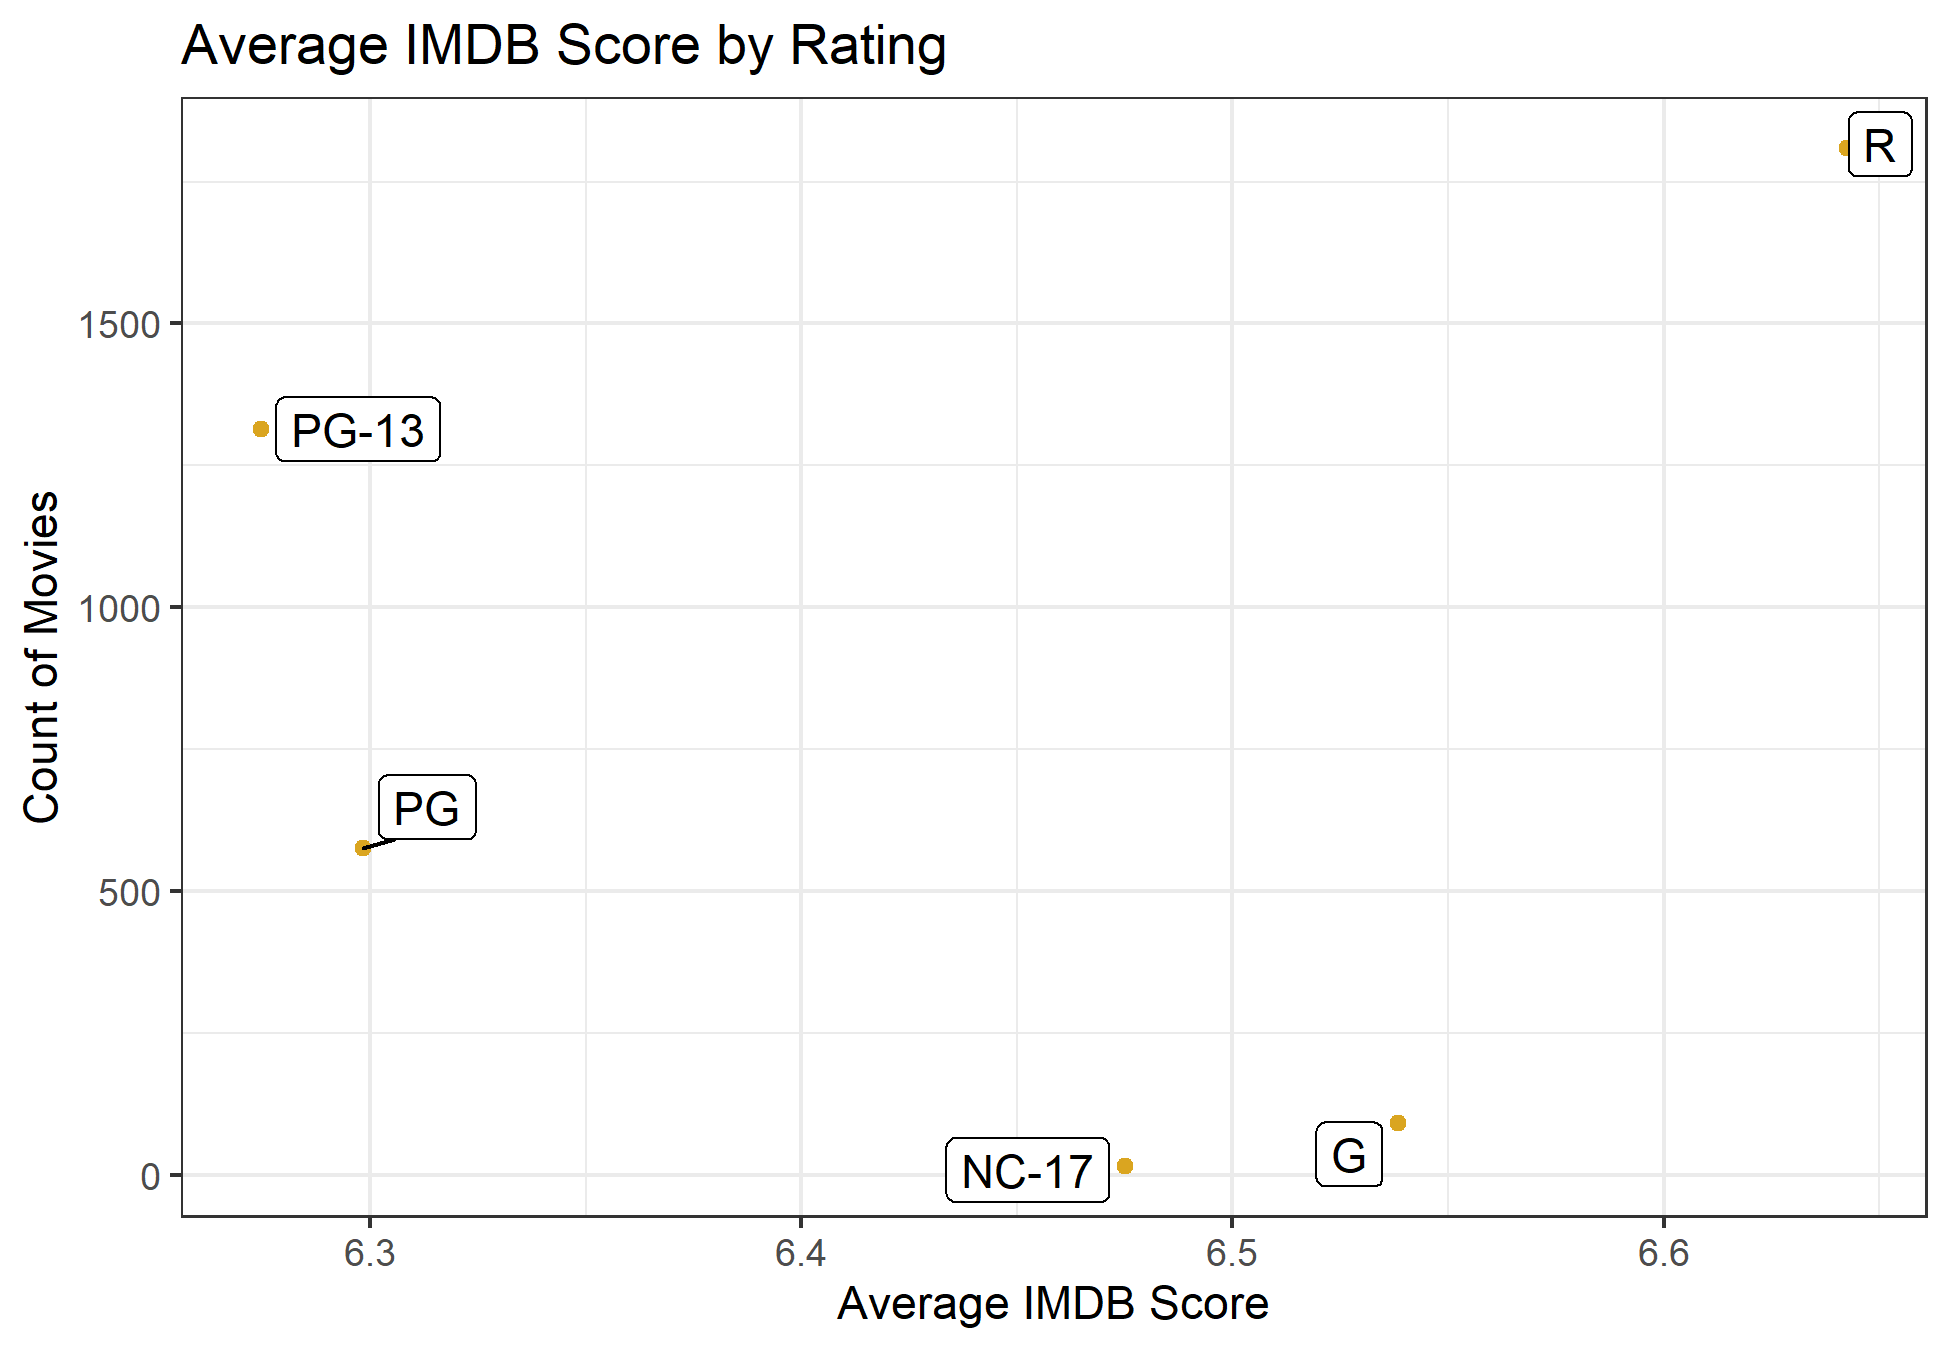
\includegraphics[width=0.75\linewidth]{IMDB_files/figure-latex/content_rating chart-1}

\hypertarget{understanding-the-distribution-of-directors-and-their-effect-on-imdb-score}{%
\subsection{Understanding the distribution of directors and their effect
on IMDB
score}\label{understanding-the-distribution-of-directors-and-their-effect-on-imdb-score}}

Directors have been grouped by the number of movies directed. The data
has been filtered to only show directors with movies directed above 10
and below 50 to remove any anomalies in the data. Directors with more
movies could have a higher fan following, credibility and success rate
possibly leading to a higher IMDB score.

According to the below distribution, even after filtering, the number of
movies for most of the directors are between 10 to 15, few are in the
range of 15 to 20 and rest two are outliers. This indicates that in this
time frame, the most naturalistic production of movies by the directors
are between 10 to 15 range. The rational can be budget, resources or
time constraints.

\begin{verbatim}
## `summarise()` ungrouping output (override with `.groups` argument)
\end{verbatim}

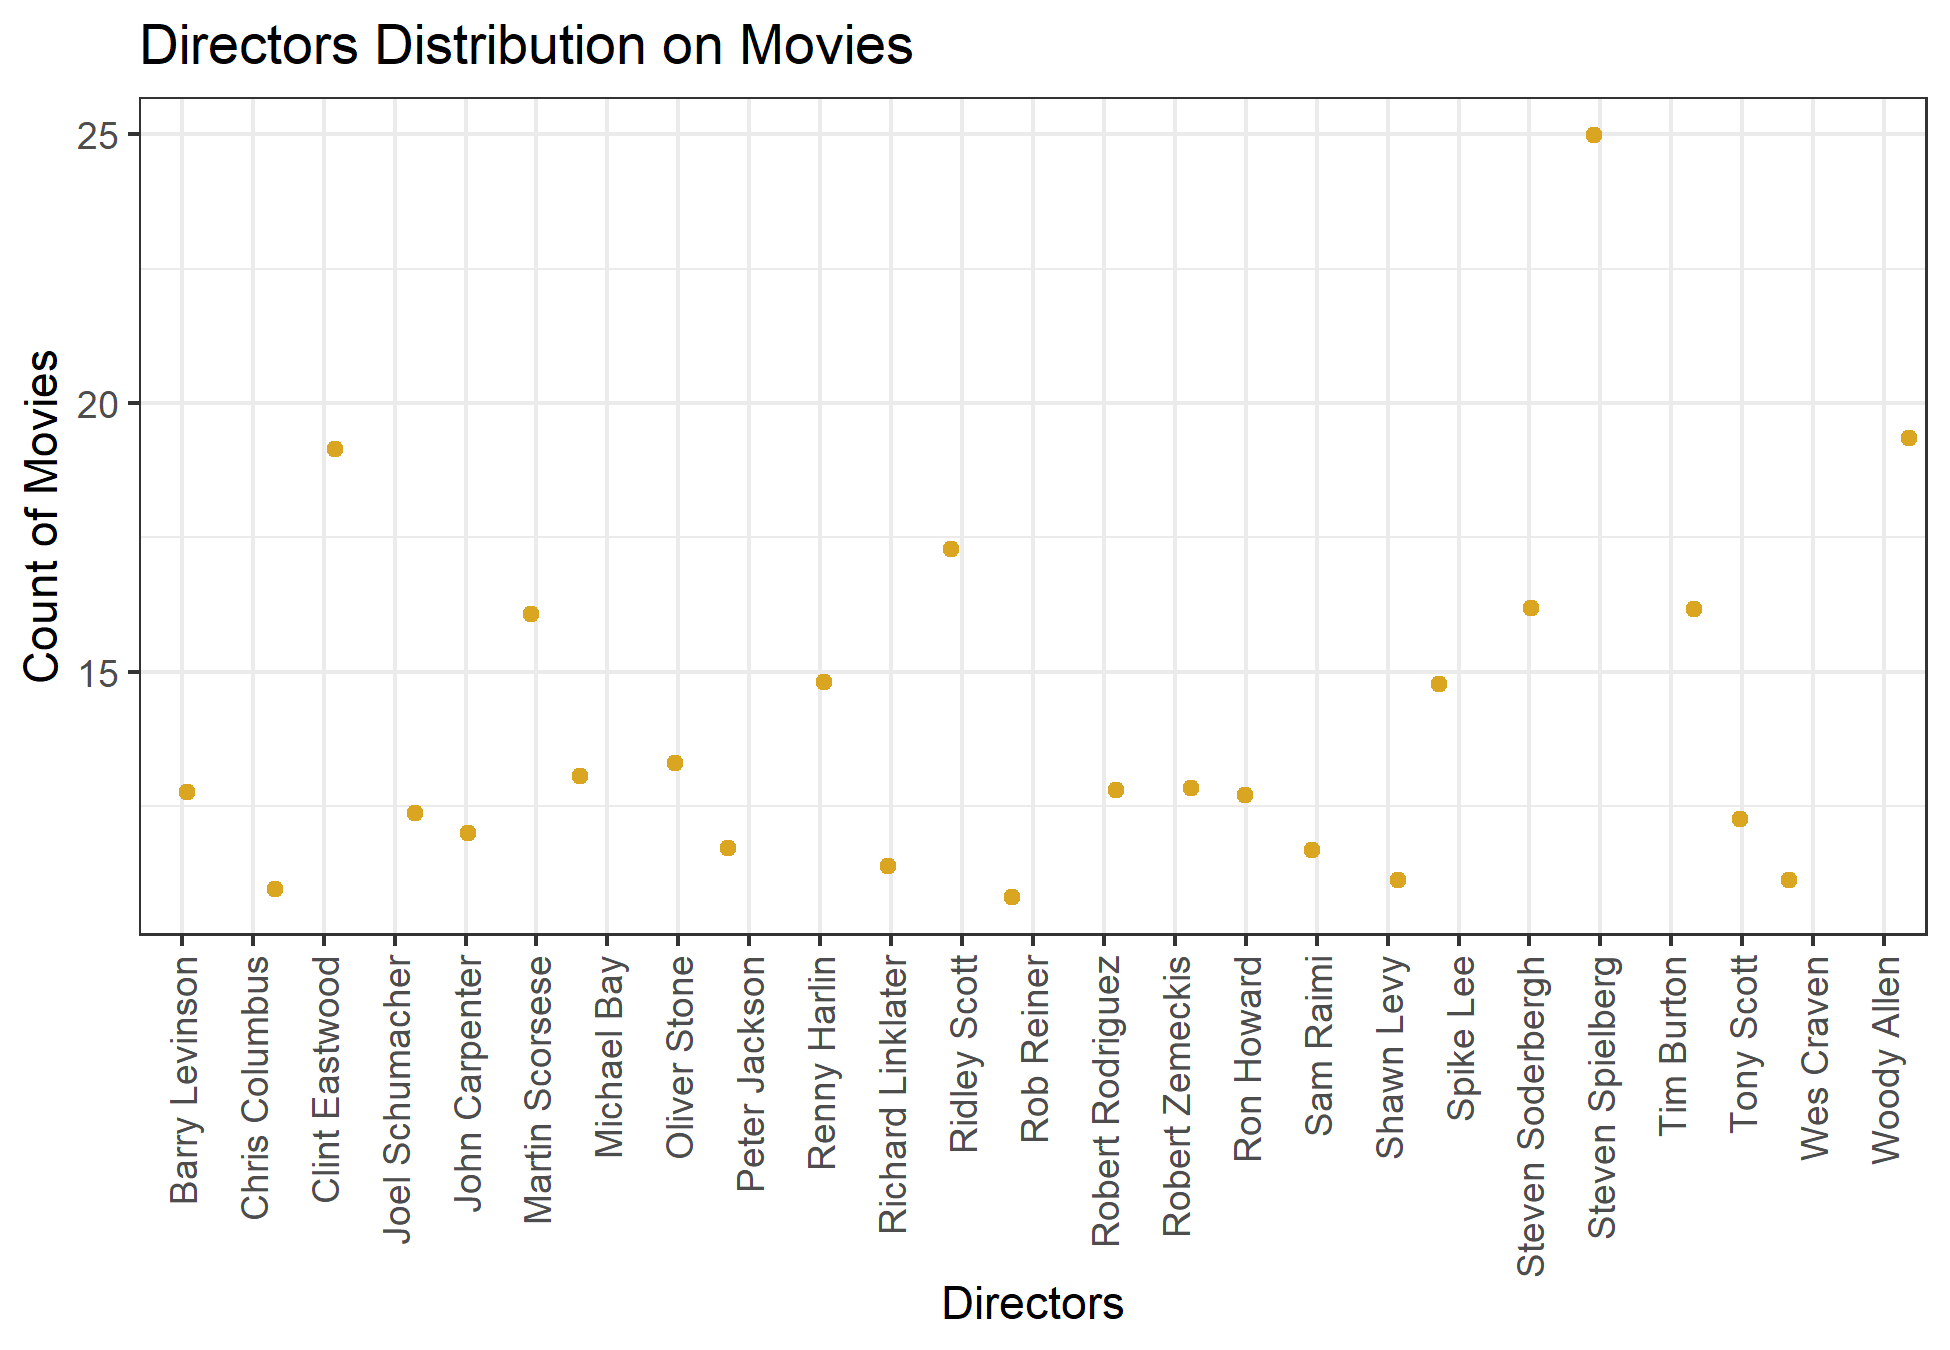
\includegraphics[width=0.75\linewidth]{IMDB_files/figure-latex/directors-1}

Only a handful of directors have over 15 movies directed in this data
set. Steven Spielberg is the only director to have \textasciitilde{} 24
movies directed. The chart below shows the average IMDB score for
directors with 15 or more directed movies. The IMDB score is above 5.5
for directors with more than 15 movies. Most directors have received a
higher IMDB score that shows the number of movies directed has a slight
impact on the IMDB score.

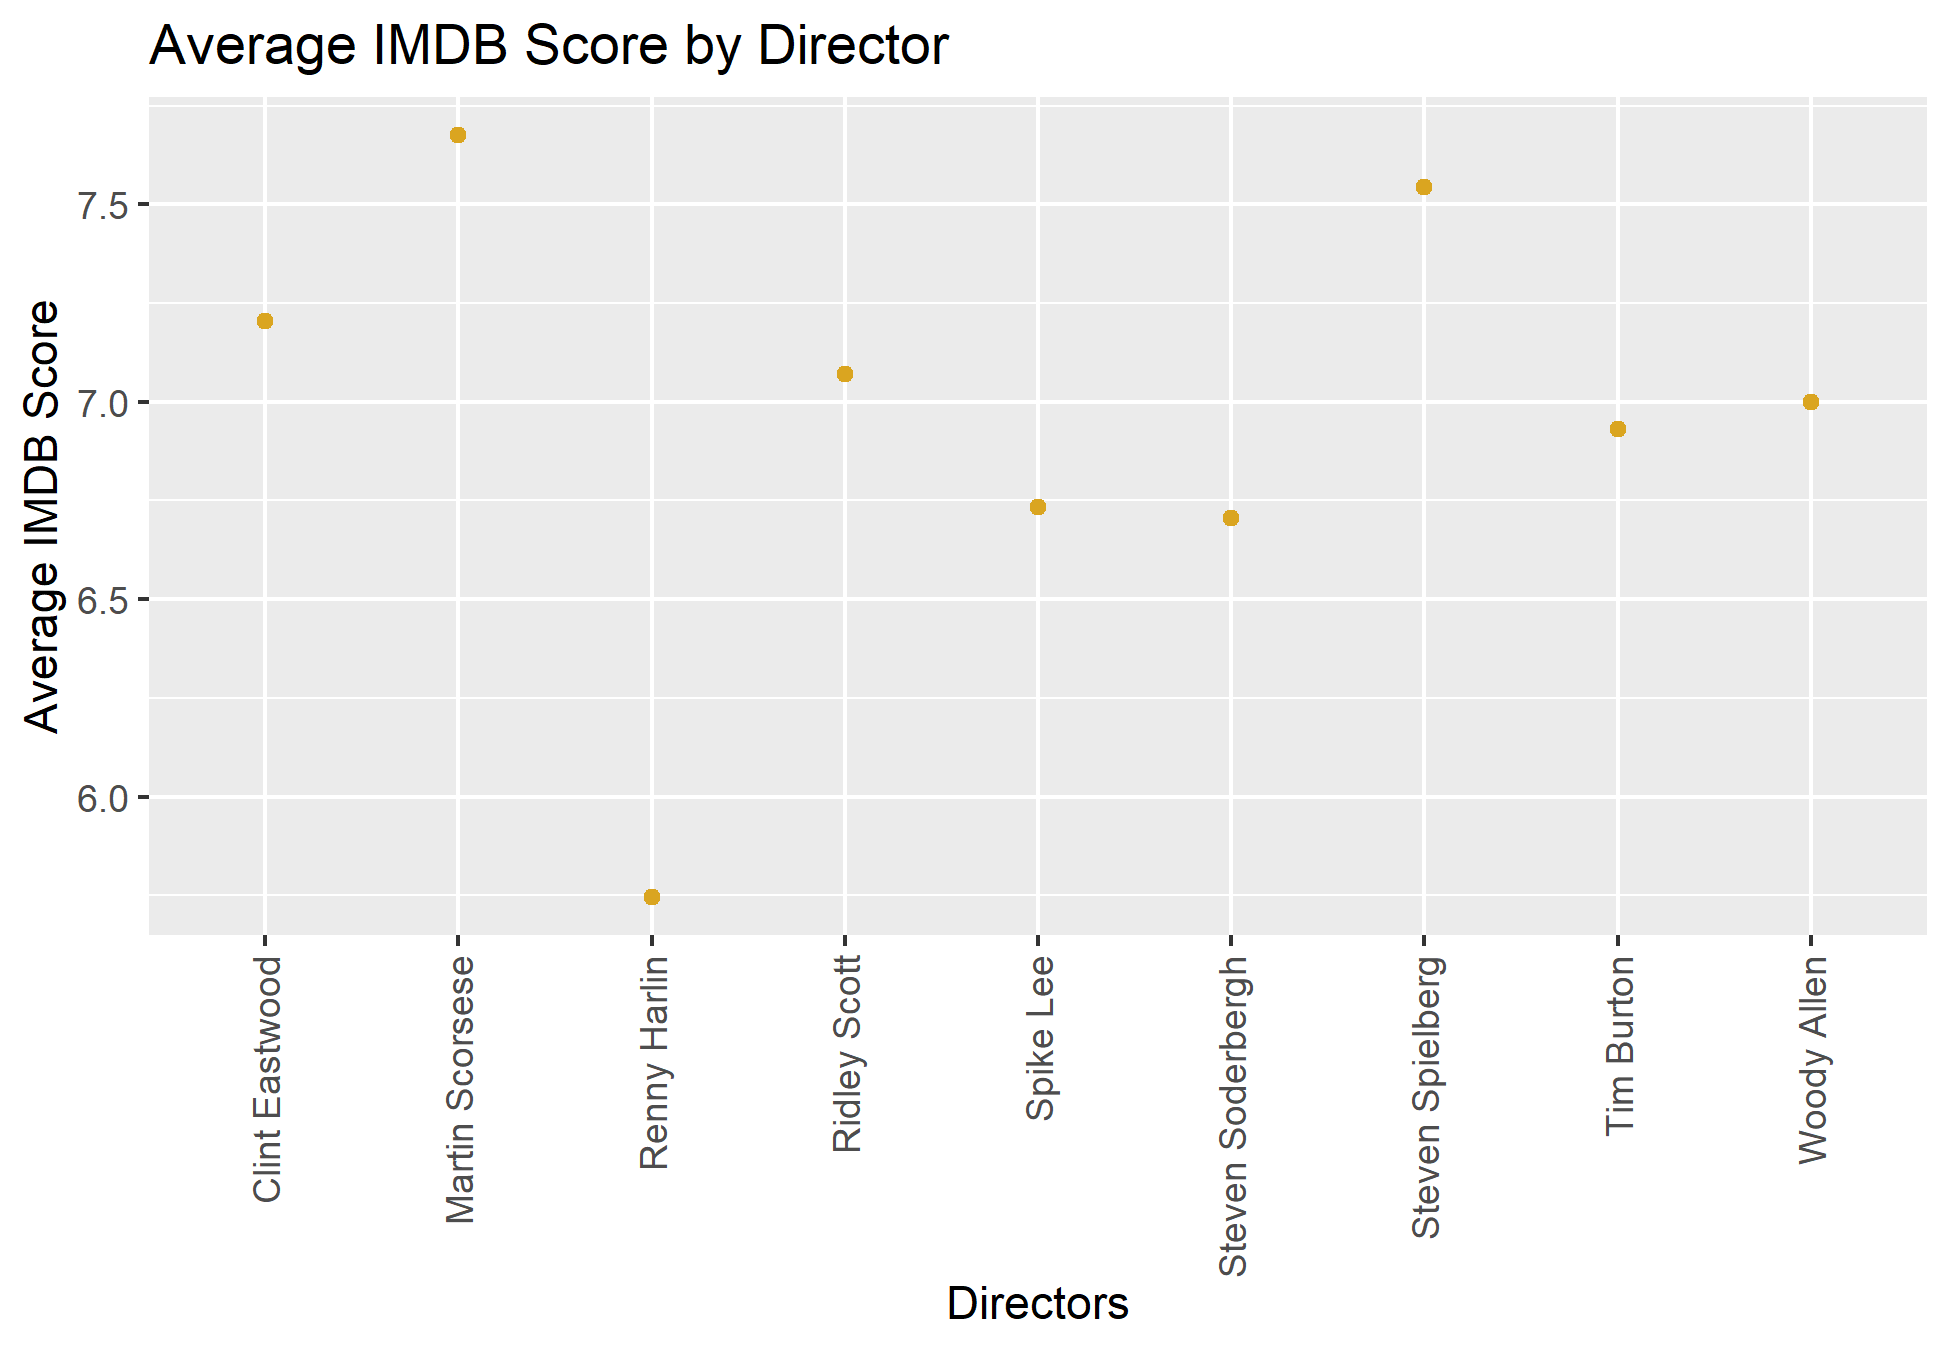
\includegraphics[width=0.75\linewidth]{IMDB_files/figure-latex/score by director-1}

\hypertarget{top-20-movies-by-imdb-score}{%
\subsection{Top 20 movies by IMDB
score}\label{top-20-movies-by-imdb-score}}

The below scatter plot shows the top 20 movies that have received the
highest IMDB scores. Most directors have more than one movie rated above
7.5 which is considered to be a good score. These movies have recieved
higher user reivews compared to other movies in the dataset. The minimum
user reviews are 1000 for these top 20 movies which is significantly
higher than the median of 205 user reviews.

1, 105, 205, 330.0793484, 392.75, 5060

\begin{verbatim}
## `summarise()` regrouping output by 'director_name' (override with `.groups` argument)
\end{verbatim}

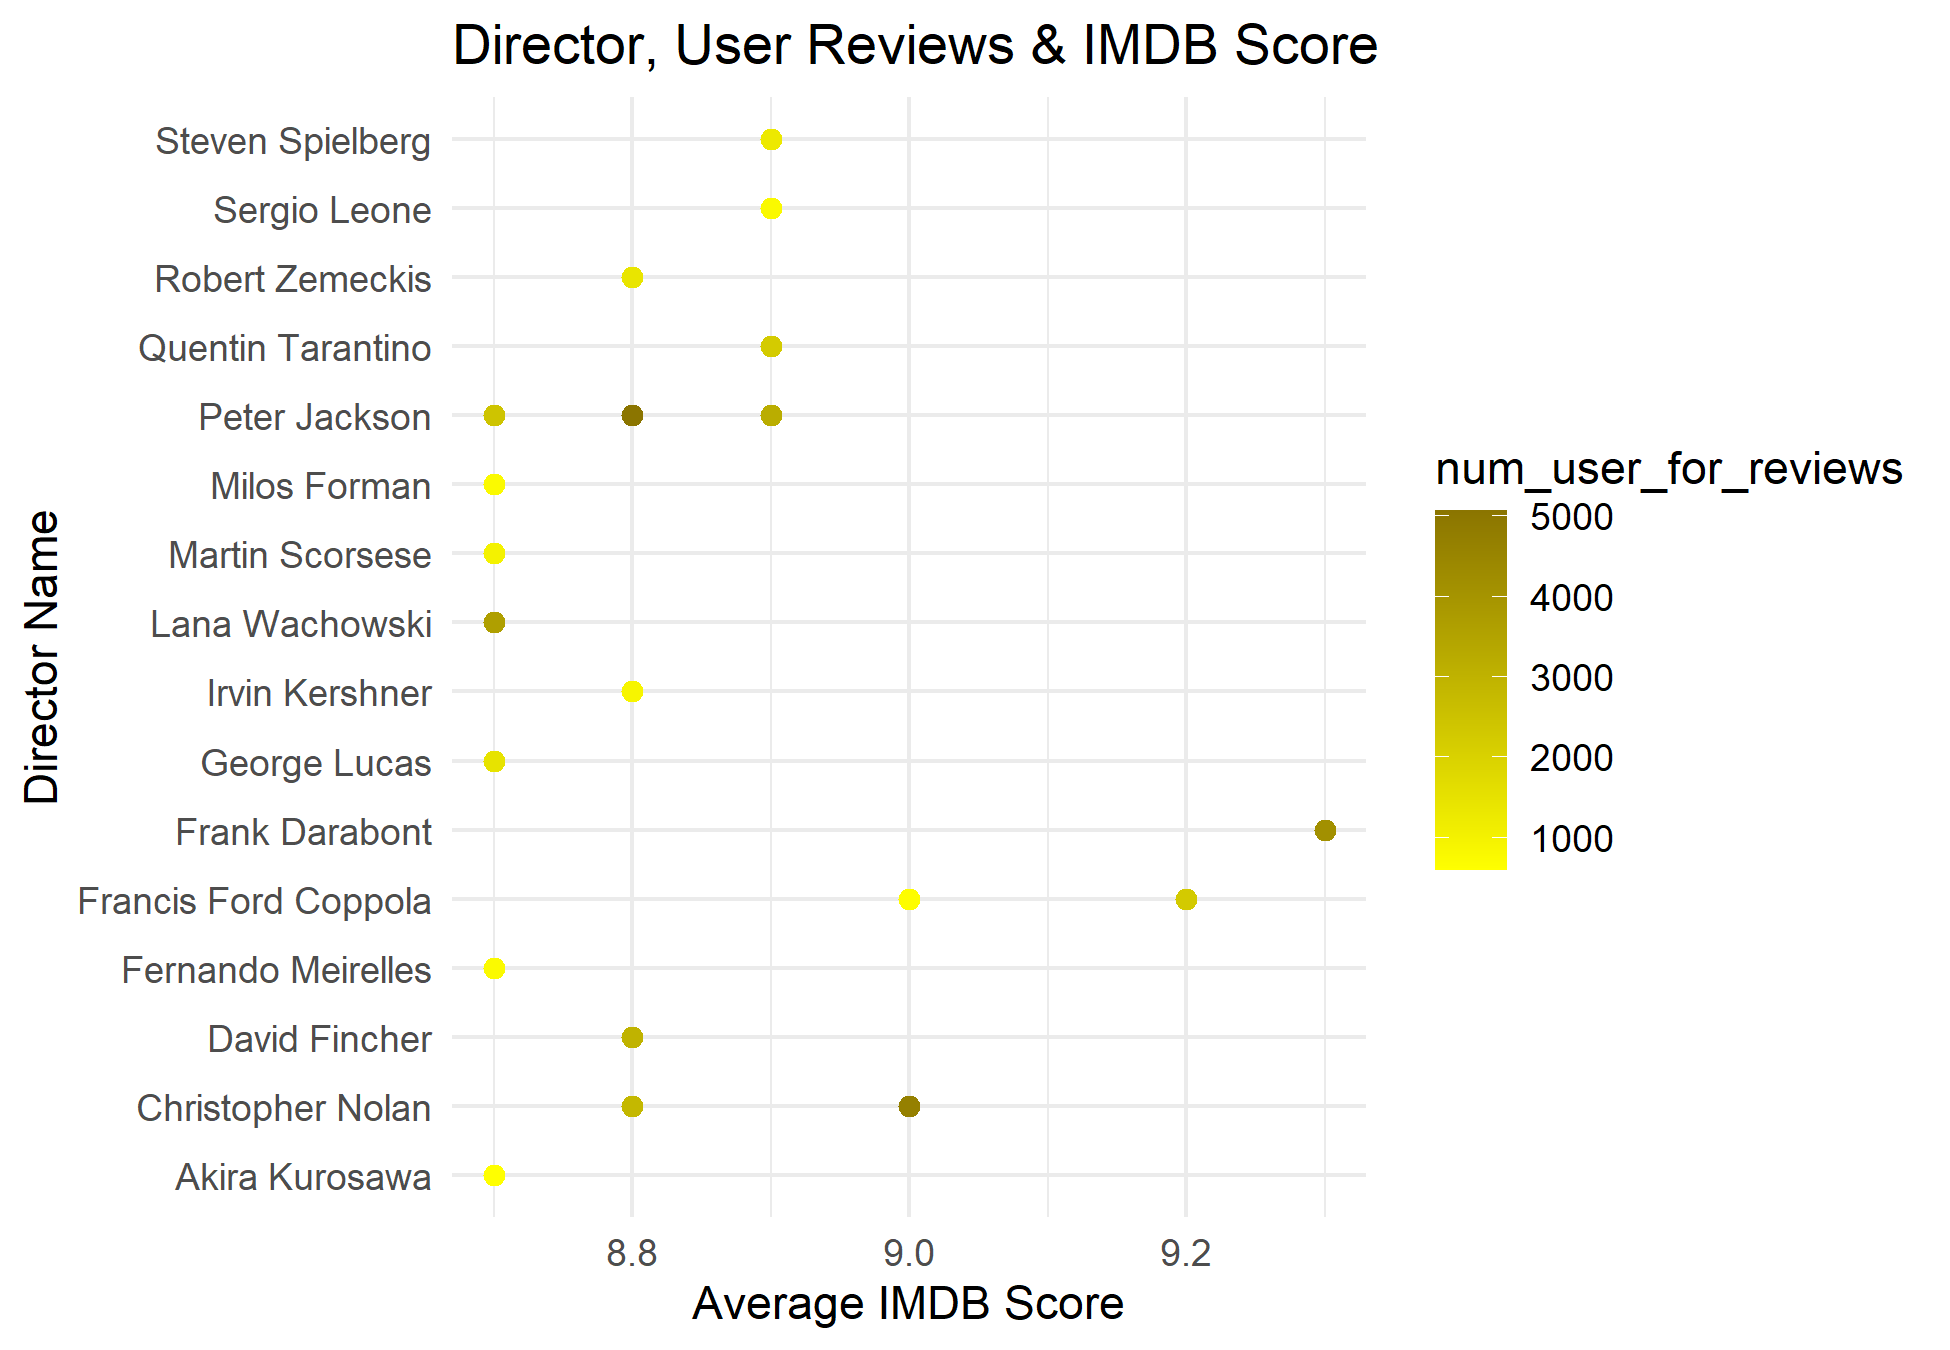
\includegraphics[width=0.75\linewidth]{IMDB_files/figure-latex/movie_by_director-1}

\hypertarget{impact-of-country-on-the-imdb-score}{%
\subsection{Impact of country on the IMDB
score}\label{impact-of-country-on-the-imdb-score}}

All countries other than U.S and U.K were grouped as others while
cleaning the data as they were significantly lower than these top two
countries. As per the below scatter plot, highest number of movies
reviewed are from the U.S followed by the U.K. Higher IMDB ratings are
seen in the U.S with the most number of user reviews. We can see the
pattern of higher scores and higher user reviews repeat in the blow plot
as well.

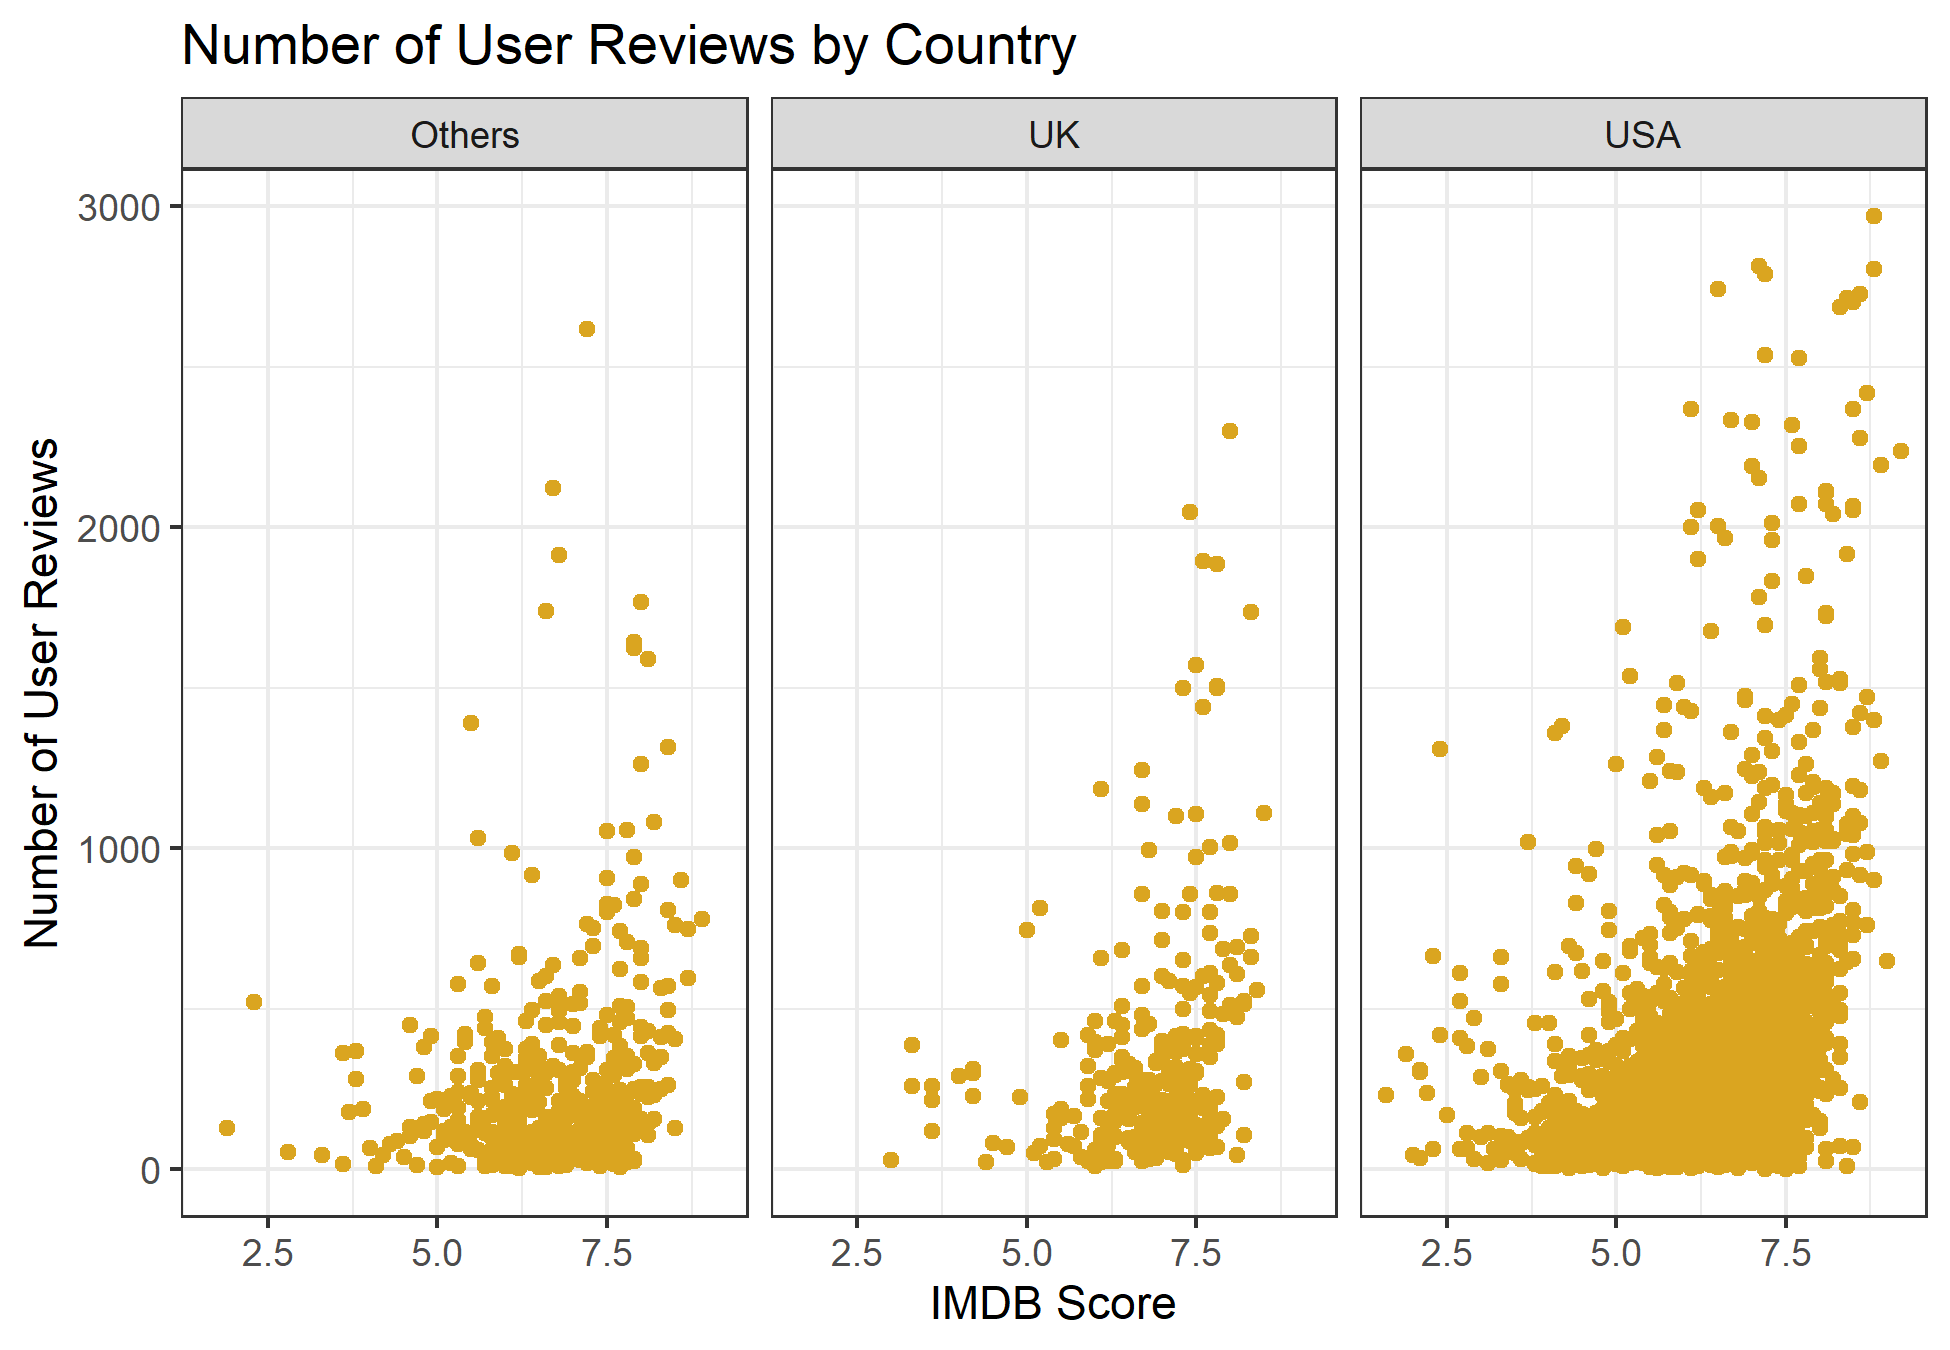
\includegraphics[width=0.75\linewidth]{IMDB_files/figure-latex/user reviews-1}
\#\# Movie durations impact on the IMDB score

The below scatter plot shows a linear relationship between IMDB score
and duration. As the duration increases the IMDB score also increases.
Most movies with a score higher 7.5 have a longer duration.

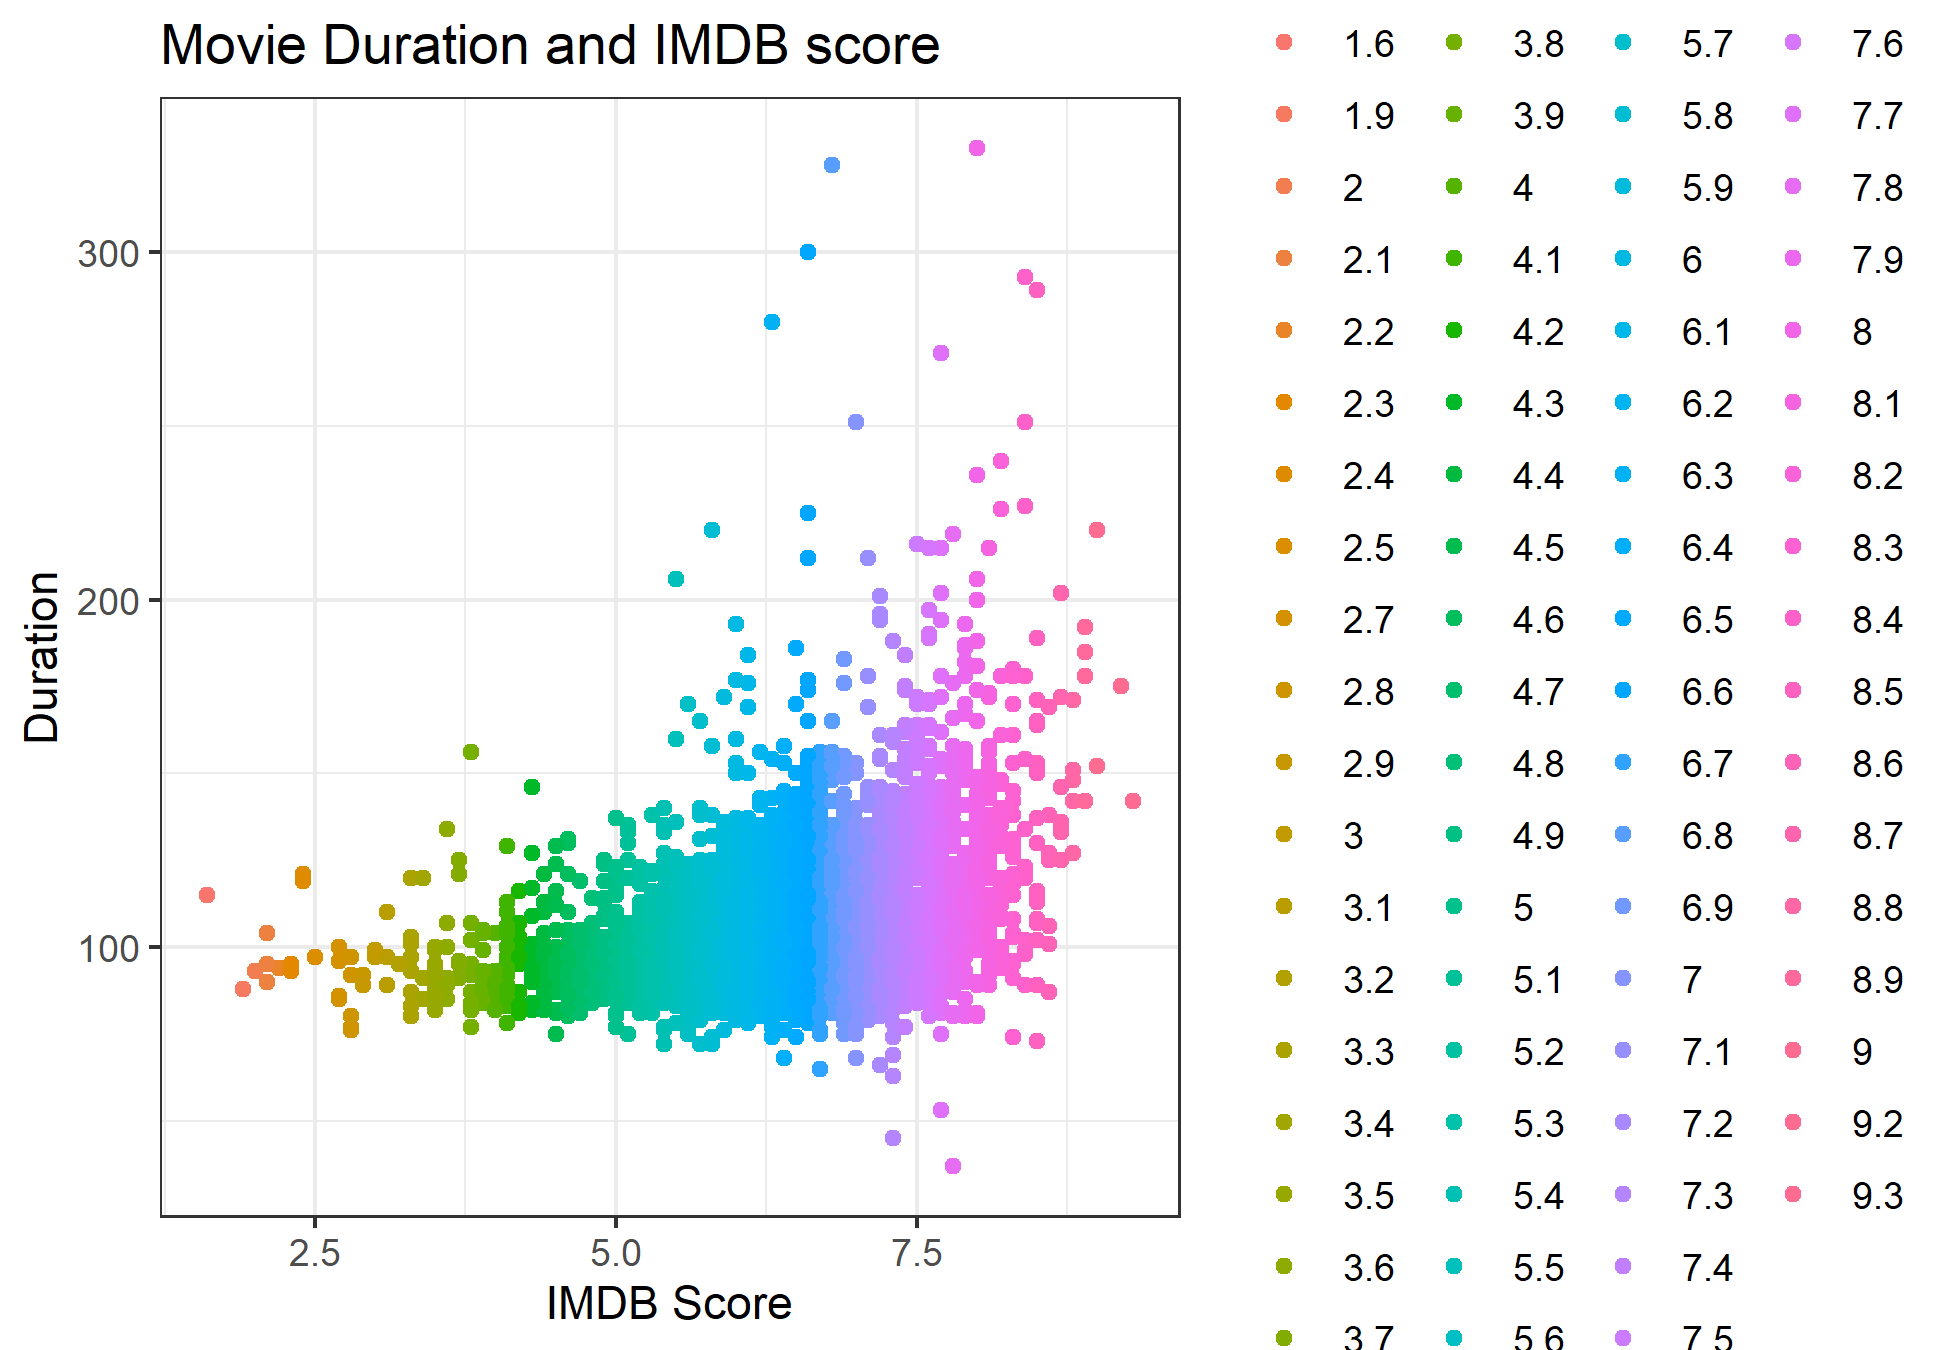
\includegraphics[width=0.75\linewidth]{IMDB_files/figure-latex/movie duration-1}

\hypertarget{impact-of-net-profit-on-imdb-score.}{%
\subsection{Impact of net profit on IMDB
score.}\label{impact-of-net-profit-on-imdb-score.}}

Movies with a net profit over 200 million have a higher IMDB rating. The
trend below shows higher net profits translates to a higher rating. It
could be assumed that the viewership for movies with higher net profits
was higher and thus, received a higher movie rating.

The movies with higher IMDB score should generate higher net profit. But
this is not always true. There are many movies that have very good IMDB
score but did not generate much profit. So, IMDB score cannot be a sole
factor to consider the net profit.

\begin{verbatim}
## `geom_smooth()` using method = 'gam' and formula 'y ~ s(x, bs = "cs")'
\end{verbatim}

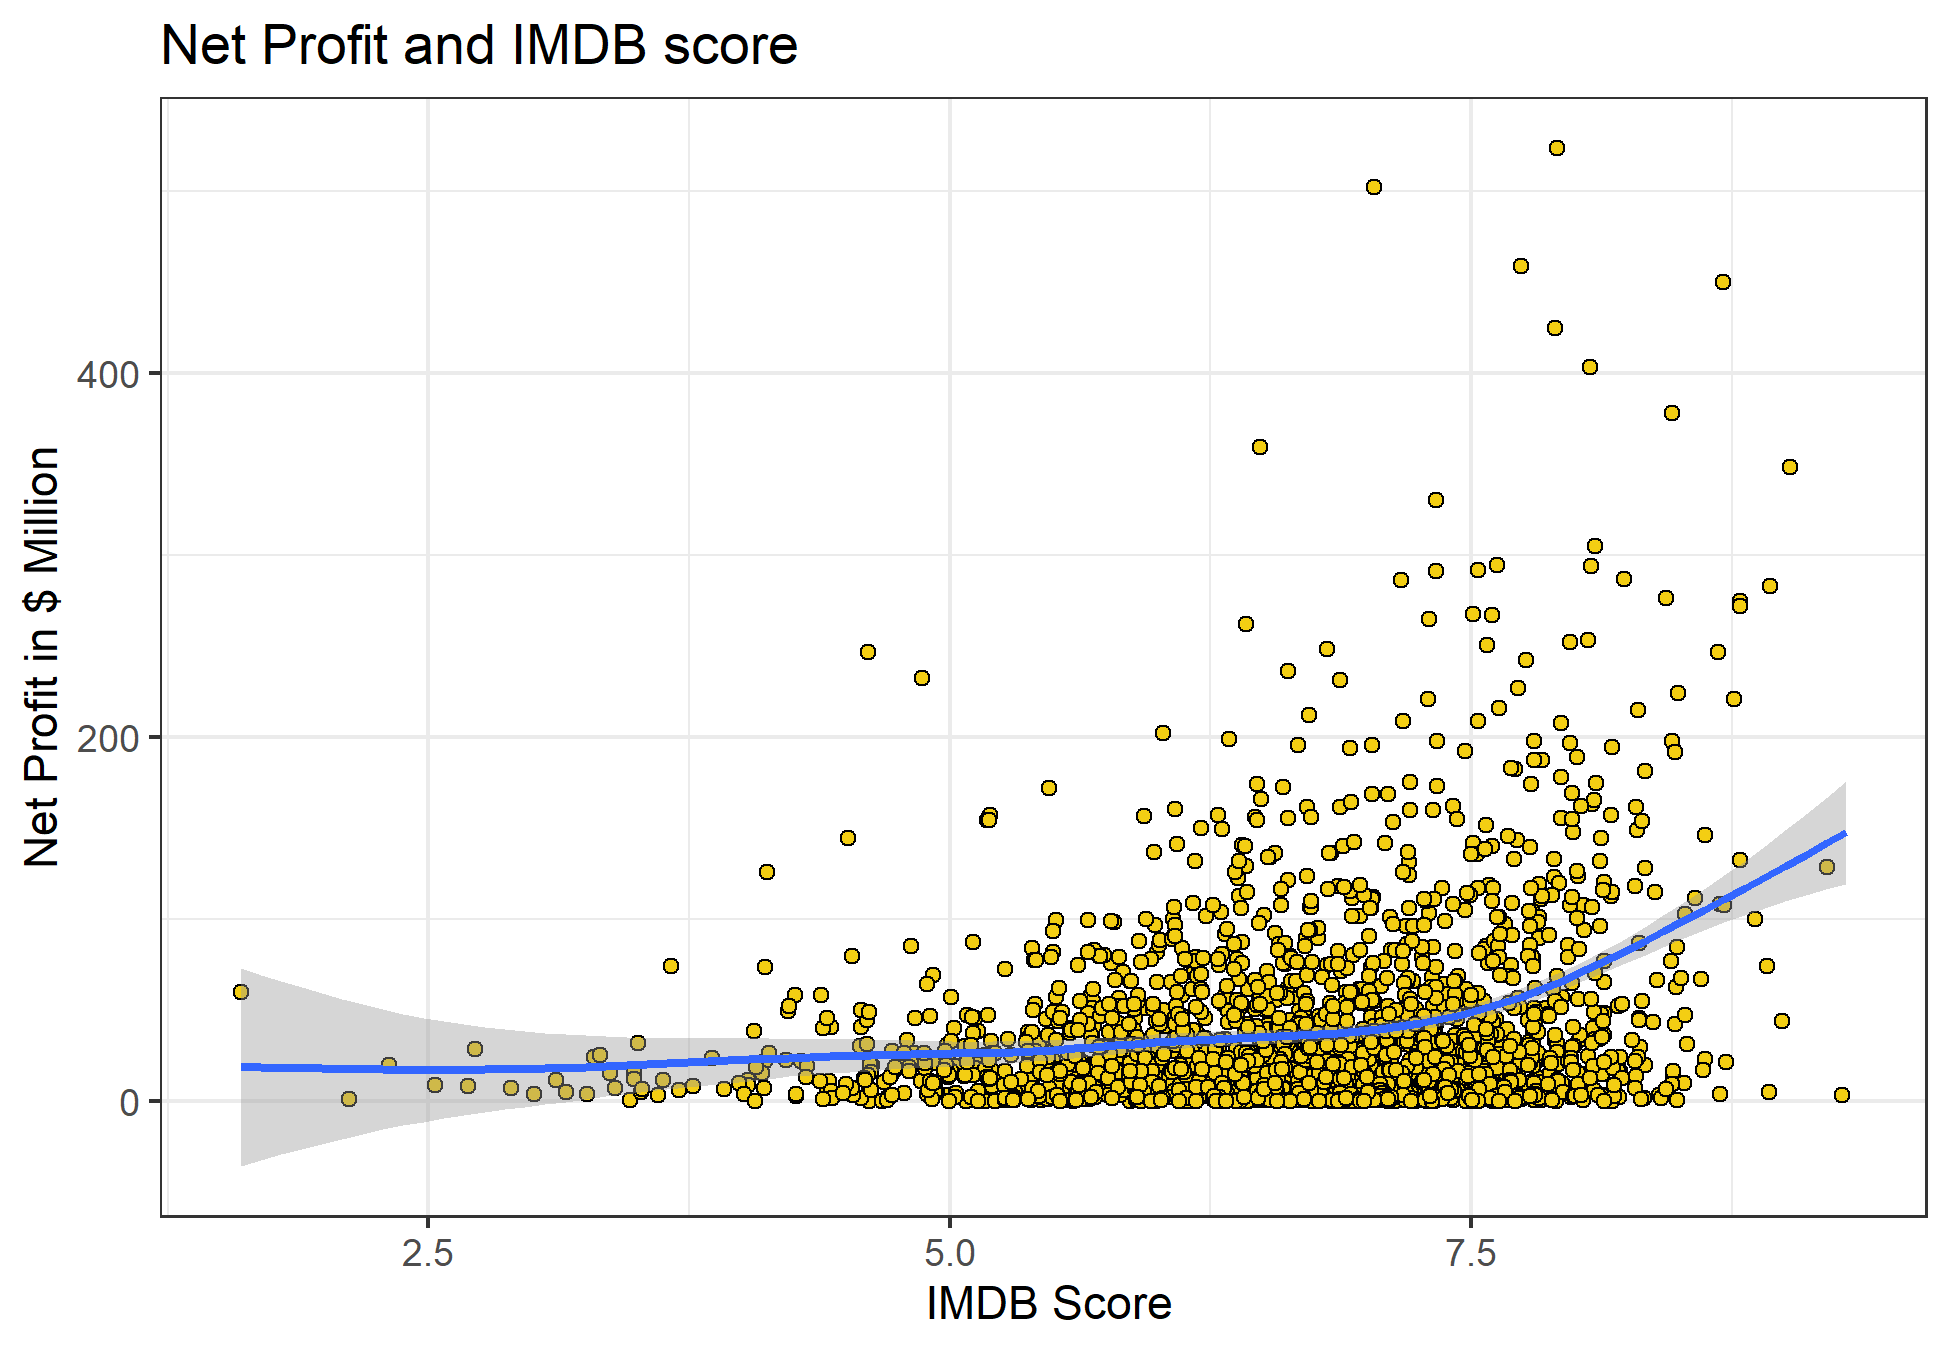
\includegraphics[width=0.75\linewidth]{IMDB_files/figure-latex/net profit-1}

\hypertarget{modeling-techniques-to-identify-the-most-important-variables-that-impact-imdb-ratings-of-the-movie}{%
\subsection{Modeling techniques to identify the most important variables
that impact IMDB ratings of the
movie}\label{modeling-techniques-to-identify-the-most-important-variables-that-impact-imdb-ratings-of-the-movie}}

Dividing the data set into two with 80\% of the data as training dataset
and the rest 20\% for testing.

\hypertarget{linear-model}{%
\section{Linear Model}\label{linear-model}}

The linear model below shows that the number of voted users, number of
critic reviews and duration has the most impact on the IMDB score. The
R-squared of 0.28 is extremely low which suggests the relationship
between these variables is not linear.

This low R-squared value indicates that IMDB score is not explaining
much in the variation of the dependent variables such as duration,
num\_voted\_users, num\_critic\_for\_reviews or movie\_facebook\_likes.
Regardless of the variable significance, this is letting us know that
the identified independent variable, even though significant, is not
accounting for much of the mean of the dependent variable.

\begin{verbatim}
## 
## Call:
## lm(formula = imdb_score ~ duration + num_voted_users + num_critic_for_reviews + 
##     movie_facebook_likes, data = IMDB_train)
## 
## Residuals:
##     Min      1Q  Median      3Q     Max 
## -4.2259 -0.5166  0.0926  0.6366  2.4831 
## 
## Coefficients:
##                         Estimate Std. Error t value Pr(>|t|)    
## (Intercept)            4.890e+00  8.486e-02  57.620   <2e-16 ***
## duration               1.105e-02  7.757e-04  14.248   <2e-16 ***
## num_voted_users        2.503e-06  1.441e-07  17.364   <2e-16 ***
## num_critic_for_reviews 4.734e-04  1.979e-04   2.392   0.0168 *  
## movie_facebook_likes   1.395e-06  1.128e-06   1.238   0.2160    
## ---
## Signif. codes:  0 '***' 0.001 '**' 0.01 '*' 0.05 '.' 0.1 ' ' 1
## 
## Residual standard error: 0.8976 on 3039 degrees of freedom
## Multiple R-squared:  0.2807, Adjusted R-squared:  0.2797 
## F-statistic: 296.4 on 4 and 3039 DF,  p-value: < 2.2e-16
\end{verbatim}

\begin{verbatim}
## [1] 0.8851699
\end{verbatim}

\hypertarget{random-forest-to-determine-the-variable-that-has-the-most-impact-on-the-imdb-score}{%
\subsection{Random Forest to determine the variable that has the most
impact on the IMDB
score}\label{random-forest-to-determine-the-variable-that-has-the-most-impact-on-the-imdb-score}}

We will be creating a random forest to identify the most important
variables on the training data. Random forest will include all the
variables from the dataset. Variables by importance are plotted below
which show us the number of voted user have the most impact on the IMDB
score.

\begin{verbatim}
##      |      Out-of-bag   |
## Tree |      MSE  %Var(y) |
##   50 |   0.5073    45.36 |
##  100 |   0.4962    44.37 |
##  150 |   0.4945    44.22 |
##  200 |   0.4932    44.10 |
##  250 |   0.4886    43.69 |
##  300 |   0.4869    43.54 |
##  350 |   0.4861    43.47 |
##  400 |   0.4842    43.30 |
##  450 |   0.4846    43.34 |
##  500 |   0.4836    43.24 |
\end{verbatim}

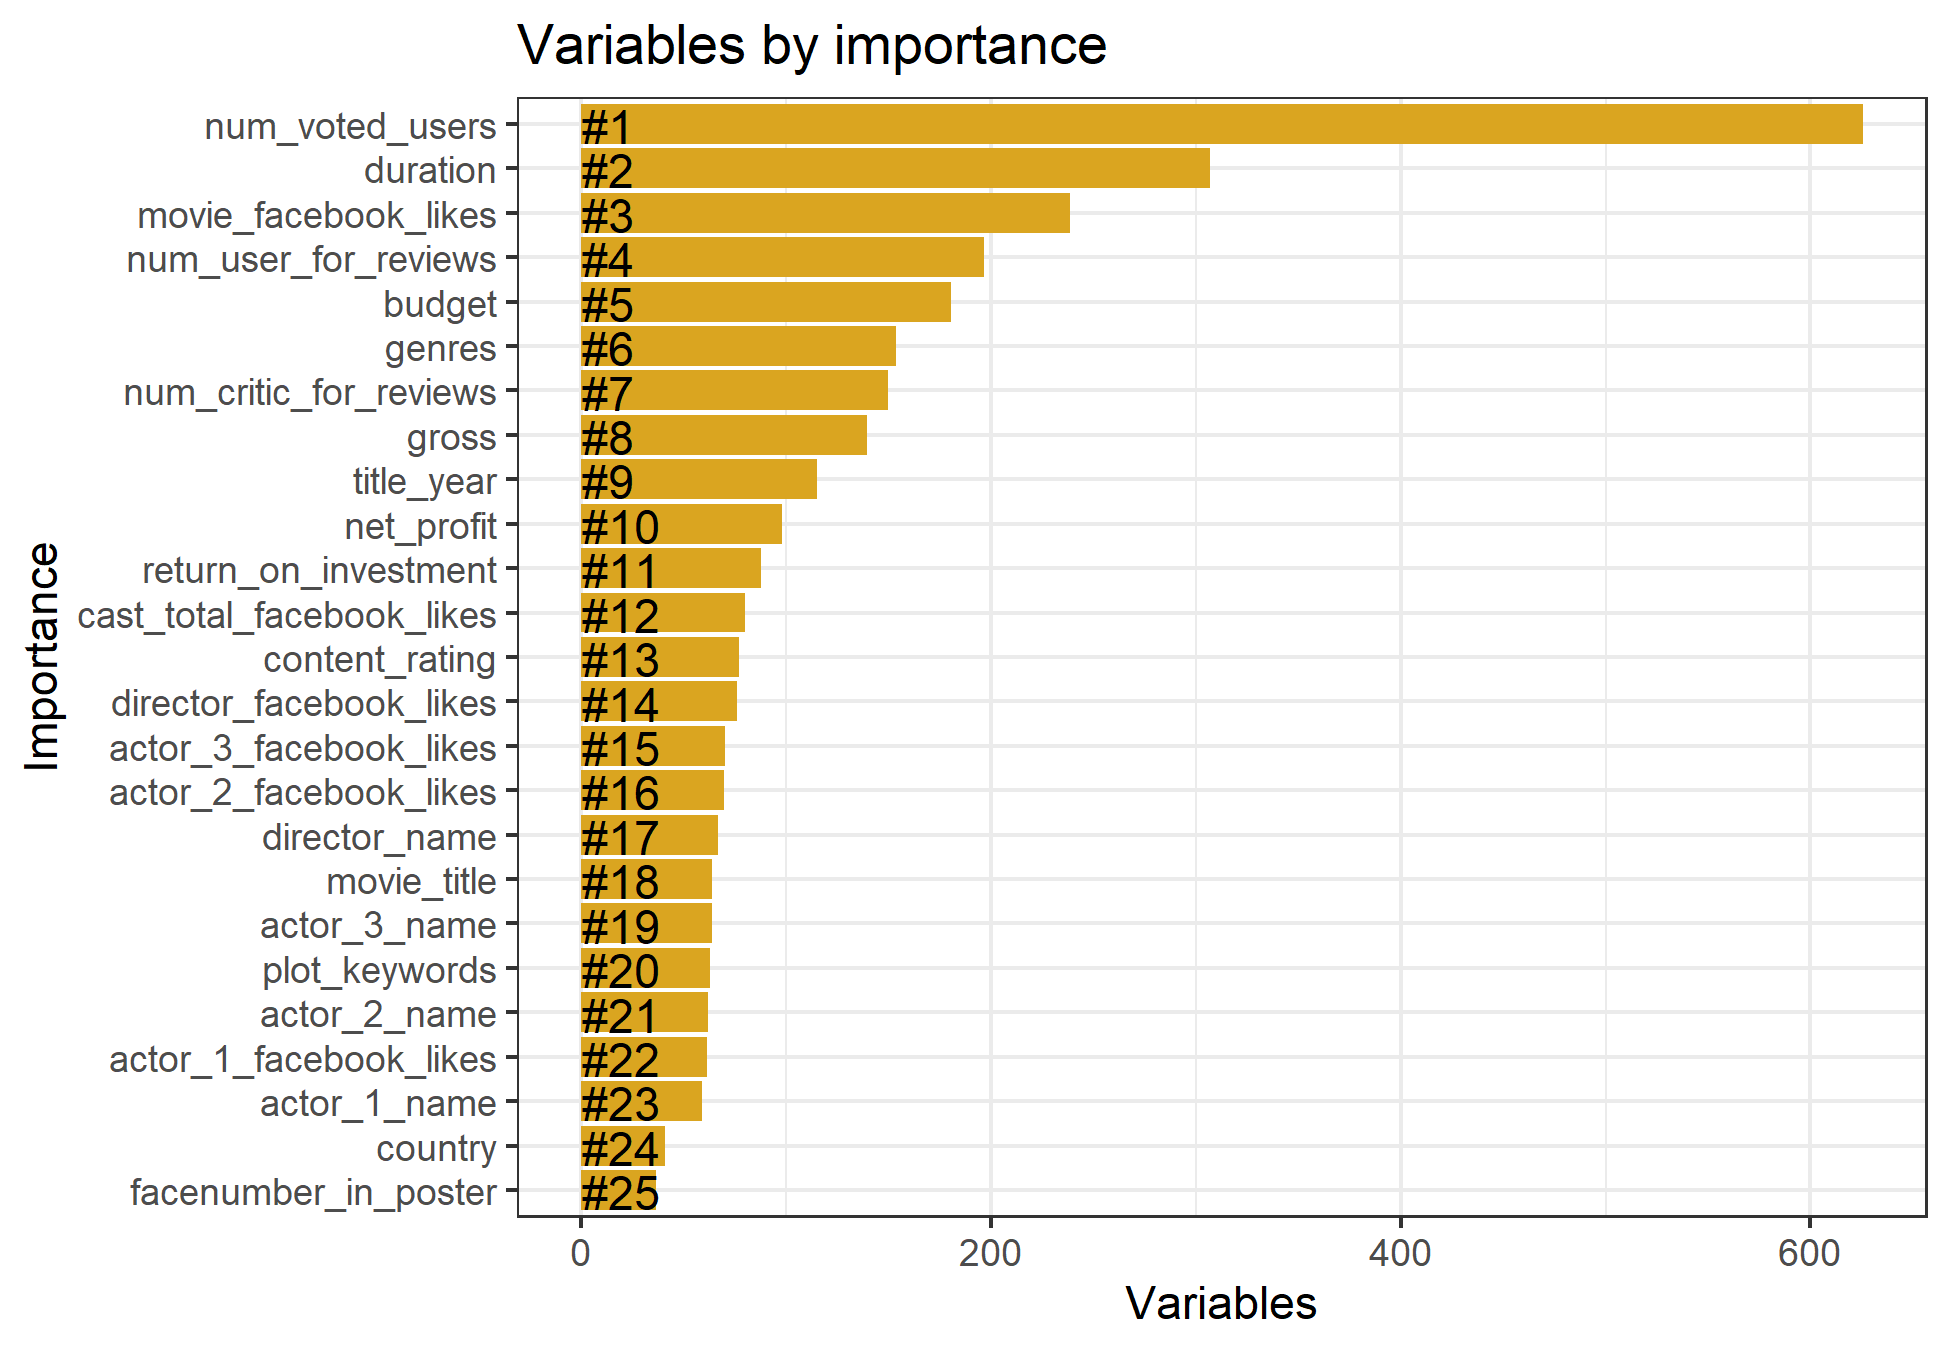
\includegraphics[width=0.75\linewidth]{IMDB_files/figure-latex/random forest-1}

The root mean squared error for the above random forest is 0.7213442
making it an average model.

\hypertarget{random-forest-with-select-variables-to-reduce-the-mean-squared-error}{%
\section{Random Forest with select variables to reduce the mean squared
error}\label{random-forest-with-select-variables-to-reduce-the-mean-squared-error}}

The mean squared error of the model below is
\texttt{mean((predict.IMDB.rf\ -\ IMDB\_test\$imdb\_score)\^{}2)} which
is lower than the previous model
\texttt{mean((predicted.rf\ -\ IMDB\_test\$imdb\_score)\^{}2)}. This
model only uses some of the most important variables which could be the
reason for a lower root mean sqaured error.

\begin{verbatim}
## [1] 0.7132754
\end{verbatim}

\begin{verbatim}
## [1] 0.5087618
\end{verbatim}

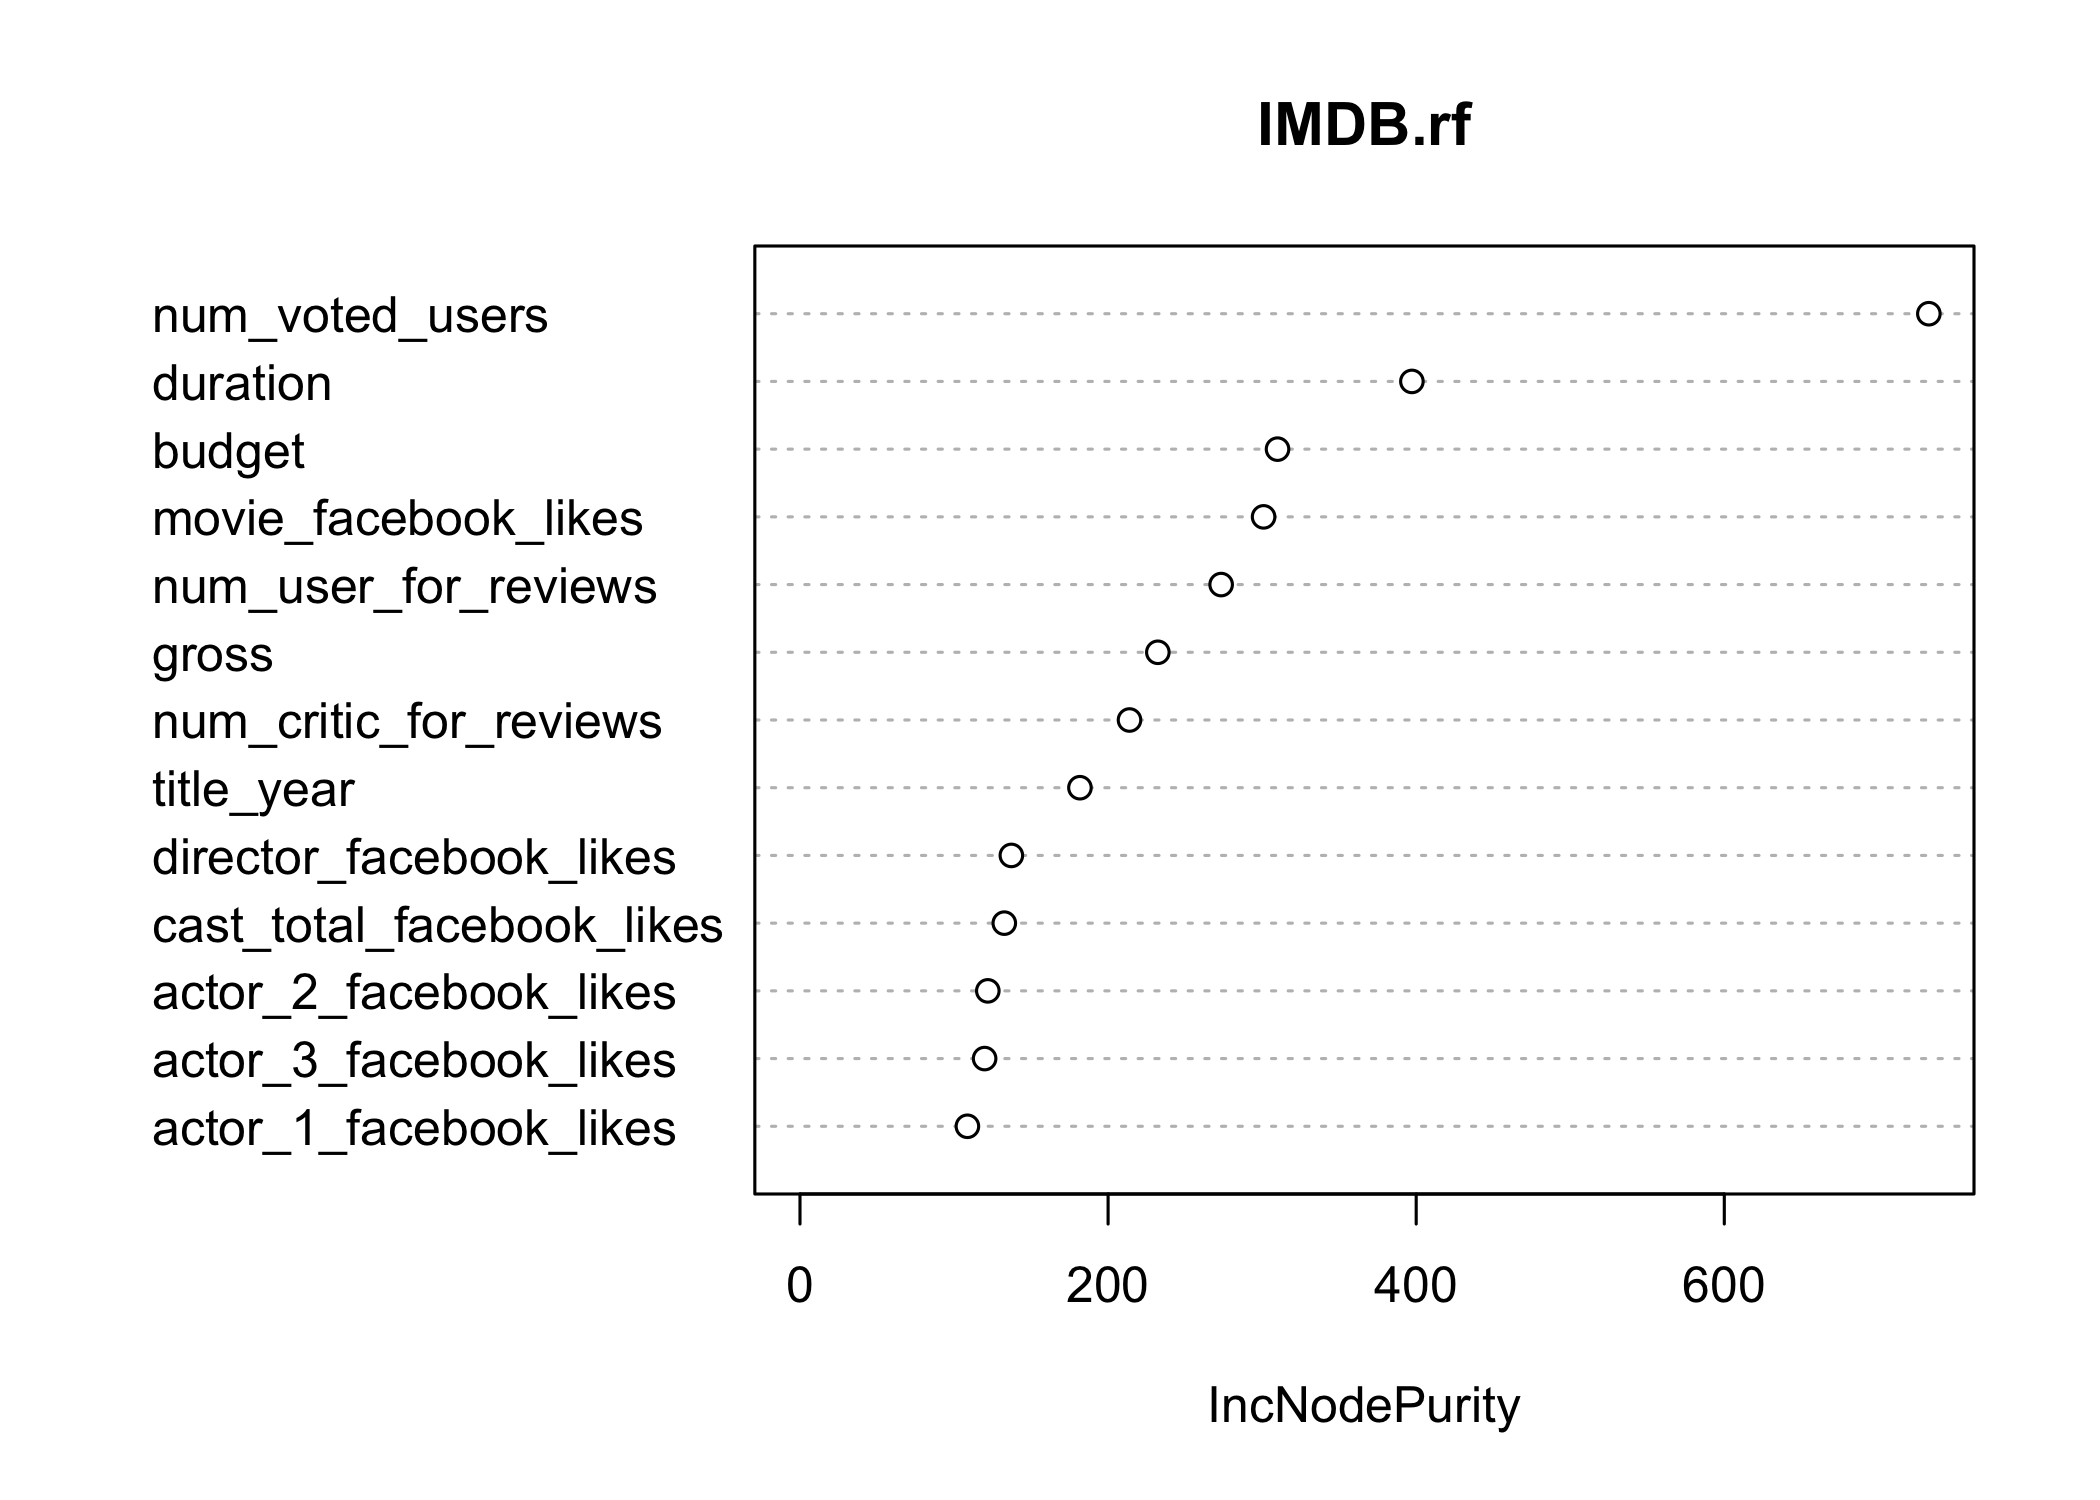
\includegraphics[width=0.75\linewidth]{IMDB_files/figure-latex/random forest II-1}

We can see that the most important variable is the number of voted
users. The reason is quite obvious because the rating only generates
when people vote or give reviews for the movies. There are a good number
of people who vote for their favorite movies which is used to calculate
the IMDB score. Second most important factor is the duration of the
movies. This is quite interesting because this is not something which is
easily guessed. However, the logical rationale behind this could be that
the long hours movies are generally high budgeted ones with popular star
cast. Therefore, the quality of the movies with longer duration are
usually better. The next factor is the facebook likes. Even though this
factor is a difficult predictor to assume, we can say that people likes
something on facebook when they truly enjoy something. So, they might
have a tendency to provide good IMDB rating as well.

The importance of next three variables, budget, genres and number of
user reviews, is very close. A high budgeted movie will typically have a
tendency to get high IMDB scores because they are usually created with
with a lot of hype and promotion. Genres also have an impact because
some genres are more attractive to users than others. Typically, action
and thriller movies are preferred to many viewers. For obvious reasons,
number of user reviews are important. These users directly rate the
movies on the IMDB website. So, certainly this will be one of the most
important factors.

\hypertarget{conclusion}{%
\section{Conclusion}\label{conclusion}}

Random Forest took into consideration all the variables from the dataset
to understand their impact on the IMDB score. Number of voted users is
the most important variable for a high IMDB score. Followed by duration
and facebook likes received by the audience. It is surprising to see,
actors and directors names were among the least impactful factors as one
would think directors and actors bring in publicity leading to a higher
viewership.

\end{document}
